%% ============================================================
%%  Opinion Homogenization via Large Language Models:
%%  Adaptive Universal Agents and the alpha/beta Ratio
%%  LXAI @ ICML 2026 workshop submission
%% ============================================================
\documentclass{article}

% Recommended, but optional, packages for figures and better typesetting:
\usepackage{microtype}
\usepackage{graphicx}
\usepackage{booktabs}

% hyperref makes hyperlinks in the resulting PDF.
\usepackage{hyperref}

% Attempt to make hyperref and algorithmic work together better:
\newcommand{\theHalgorithm}{\arabic{algorithm}}

% LXAI workshop style (blind/review mode by default).
\usepackage{lxai}

% For theorems and such
\usepackage{amsmath}
\usepackage{amssymb}
\usepackage{amsthm}

%% --- Theorem-like environments (section-scoped, sharing theorem counter) ----
\theoremstyle{plain}
\newtheorem{theorem}{Theorem}[section]
\newtheorem{proposition}[theorem]{Proposition}
\newtheorem{lemma}[theorem]{Lemma}
\newtheorem{corollary}[theorem]{Corollary}
\theoremstyle{definition}
\newtheorem{definition}[theorem]{Definition}
\theoremstyle{remark}
\newtheorem{remark}[theorem]{Remark}

%% --- Notation shorthands ----------------------------------------------------
\newcommand{\bx}{\mathbf{x}}
\newcommand{\bw}{\mathbf{w}}
\newcommand{\bz}{\mathbf{z}}
\newcommand{\bone}{\mathbf{1}}
\newcommand{\xUA}{x_{\mathrm{UA}}}
\newcommand{\xbar}{\bar{x}}
\newcommand{\mbar}{\bar{m}}
\newcommand{\ubar}{\bar{u}}
\newcommand{\Ni}{\mathcal{N}_i}
\newcommand{\Var}{\mathrm{Var}}

%% The \icmltitle you define below is probably too long as a header.
%% Therefore, a short form for the running title is supplied here:
\icmltitlerunning{Opinion Homogenization via Large Language Models}

\begin{document}

\twocolumn[
\icmltitle{Opinion Homogenization via Large Language Models}

\begin{icmlauthorlist}
\icmlauthor{Anonymous Author(s)}{anon}
\end{icmlauthorlist}
\icmlaffiliation{anon}{Anonymous Institution}
\icmlcorrespondingauthor{Anonymous Author}{anon.email@domain.com}

\icmlkeywords{opinion dynamics, cultural homogenization, universal agent, phase transition, large language models, AI governance}

\vskip 0.3in
]

\printAffiliationsAndNotice{}  % for blind/review submission

%% ------------------------------------------------------------
\begin{abstract}
Large language models (LLMs) are increasingly deployed as universal conversational partners, interacting with millions of users at once. We study the collective consequences with an opinion dynamics model in which one or more \emph{Universal Agents} (UAs) interact with every member of a population and adapt toward it in turn.  The model extends Hegselmann--Krause bounded-confidence dynamics in three directions: the AI can adapt toward its users (with the fixed-AI case as a special limit), several AIs can serve different population partitions and adapt either globally or locally, and individual users may rely on the AI with different strengths. In simulations with $N=100$ agents, the population exhibits a sharp transition from multiple opinion clusters to consensus when AI reliance crosses a small threshold.  With multiple adaptive AIs, global adaptation drives all AIs---and the entire population they serve---to a single shared consensus, while local adaptation preserves a stable multi-cluster equilibrium with closed-form partition-specific consensus values. These results suggest that homogenization risk depends not only on model bias, but also on the rate at which an AI adapts to its users, and on whether an ecosystem of AIs adapts globally or locally.
\end{abstract}

%% ============================================================
\section{Introduction}
\label{sec:intro}

The last several years have witnessed the rapid diffusion of large
language models (LLMs) into everyday life. Writing assistance, search,
tutoring, therapy, coding, and creative work now routinely involve AI
systems whose outputs are consumed by hundreds of millions of users
\citep{sharma2024}.  This pattern differs qualitatively from any
prior technological intervention in opinion and culture: a single
system---or a small number of systems sharing similar training corpora
and value representations---interacts simultaneously with a substantial
fraction of an entire population, at every session, across every
domain of discourse.

This configuration raises a pressing theoretical question: \emph{does
universal AI interaction induce homogenization of opinion and culture
at the population level?}  Beyond a yes/no, two follow-up questions
matter for design and policy. First, since real LLMs are not static
oracles but are continually retrained on user-influenced data, how does
the \emph{rate} at which an AI adapts to its users trade off against
the strength of its influence on them?  Second, when several different
AI systems coexist in the same population, does that diversity persist,
or does mutual exposure---through training corpora, shared benchmarks,
and overlapping user bases---collapse the ecosystem to a single
effective viewpoint?

Classical opinion dynamics provides tools for studying how opinions
evolve through peer interaction \citep{castellano2009}, but the
existing toolkit does not directly capture the LLM scenario.  Zealot
models \citep{mobilia2003, mobilia2007} introduce fixed-opinion agents,
but zealots only interact with local neighborhoods.  Stubborn-agent
analyses \citep{acemoglu2013binary} preclude consensus in binary
dynamics, again only through a subset of edges.  Mass-media models
\citep{crokidakis2014, chica2023} come closest---a single source
broadcasts to the entire population---but they are typically studied
through simulation, focus on binary or Potts opinions, and do not
allow the source itself to co-evolve with its audience.  None of
these frameworks provides the combination of analytic tractability,
continuous opinions, and bidirectional adaptation that the LLM
scenario demands.

\paragraph{Contributions.}
The paper is organized around three main results.  As a preliminary,
we observe that in linear DeGroot dynamics the adaptive UA framework
collapses to a standard $(N+1)$-agent DeGroot consensus---the UA is
itself a DeGroot agent with a specific weight pattern---which yields
the closed-form value
$x^*=(\beta\,\mbar(0)+\alpha\,u(0))/(\alpha+\beta)$ for any
$\alpha,\beta>0$ by the classical theorem.  We use this expression as
an illustrative template throughout; the substantive contributions
concern regimes in which the dynamics are not reducible to standard
DeGroot.
First, in Hegselmann--Krause (HK) dynamics---where peer averaging
alone produces several persistent opinion clusters---we show that a
common AI reference point dissolves those clusters by pulling them
into mutual confidence range, with a critical coupling on the order
of $10^{-3}$ in the parameter regime we test.  This is the
qualitatively new regime: the AI does not merely accelerate something
the population would have done anyway, it changes the asymptotic
structure from $K>1$ clusters to a single cluster.
Second, we extend the model to multiple adaptive UAs that each
interact with a distinct population partition.  In that setting,
globally adaptive UAs eventually converge to a common opinion,
collapsing the population to a single shared consensus that weights
each AI's initial opinion by its share-to-adaptation ratio
$p_j/\beta_j$, while locally adaptive UAs preserve multiple
partition-specific equilibria
$x_j^*=(\beta_j\,\mbar_j(0)+\alpha\,u_j(0))/(\alpha+\beta_j)$.
Third, when reliance on the AI varies across the population, heavy
users homogenize first and may seed a cascade that pulls less-reliant
users along through ordinary peer dynamics, producing a stratified
convergence pattern.
Together, these results separate three questions that are often
conflated in discussion of LLM deployment: when AI breaks social
bubbles, when an ecosystem of different models truly preserves
pluralism, and how unequal AI usage stratifies the population.

%% ============================================================
\section{Related Work}
\label{sec:related}

\subsection{Opinion Dynamics and Influential Agents}

The mathematical study of opinion evolution began with
\citet{degroot1974}, whose linear model updates beliefs as weighted
averages encoded in a row-stochastic matrix~$W$, converging to a
consensus determined by the stationary distribution of~$W$.
\citet{friedkin1990} extended DeGroot with stubbornness, producing
persistent disagreement.  Bounded-confidence
models---\citet{deffuant2000} (pairwise, stochastic) and
\citet{hegselmann2002} (synchronous, neighborhood averaging)---capture
opinion clustering: large confidence bound $\varepsilon$ yields
consensus, small $\varepsilon$ leaves agents isolated
\citep{bernardo2024,castellano2009}.

Alongside these peer-interaction frameworks, \citet{mobilia2003,
mobilia2007} showed that even a small committed minority (``zealots'')
can sustain or rapidly spread a minority opinion.
\citet{acemoglu2013binary} established that stubborn agents preclude
consensus in binary dynamics.  A crucial distinction separates zealots
from our UA: zealots interact only with local neighborhoods, whereas
the UA has \emph{direct} influence on every assigned agent at every
step, and, in our adaptive variant, also \emph{updates} based on
those interactions.

\subsection{Media Models and AI-Driven Homogenization}

Closer to our setting, \citet{crokidakis2014} modeled mass media as
an external field in a continuous-opinion model, finding that even
weak coupling significantly narrows the opinion distribution and can
eliminate multi-cluster configurations.  \citet{chica2023} proposed a
unified framework distinguishing individuals, media, and influencers
on different time scales.  Our adaptive UA model extends this line
in two key directions: (i) we allow the UA to adapt to the population
(parameter $\beta$), creating a co-evolutionary system not studied in
prior media-agent models; and (ii) we derive analytical results
beyond simulation, including a closed-form fixed point and a
generalization to multiple co-evolving UAs.

Recent empirical research documents AI-driven opinion homogenization
directly.  \citet{sharma2024} found that LLM-powered search creates
generative echo chambers, reinforcing user biases.
\citet{zhang2025} showed that participants using LLMs produce
markedly more homogeneous survey responses.  \citet{daryani2026}
characterize LLMs as ``homogenizing engines'' exceeding all prior
technologies in speed and scale, identifying a self-reinforcing
feedback loop---LLM-generated text enters future training corpora,
compounding cultural drift across model generations---that our
adaptive UA model captures formally.  Our paper provides the
mathematical scaffolding: a precise co-evolutionary model, proved
theorems, and simulation validation establishing \emph{when} and
\emph{by how much} universal AI interaction induces cultural
homogenization, and \emph{how} the ratio $\alpha/\beta$ controls the
outcome.

%% ============================================================
\section{Model}
\label{sec:model}

We work throughout with $N$ agents indexed $i=1,\ldots,N$, each
holding a scalar opinion $x_i(t)\in\mathbb{R}$ at discrete time
$t=0,1,2,\ldots$ (the extension to $d>1$ is discussed in
Section~\ref{sec:discussion}).  The population mean at time~$t$ is
$\xbar(t)=\frac{1}{N}\sum_i x_i(t)$.  Peer interactions are encoded
in a row-stochastic weight matrix $W=[w_{ij}]$ with $w_{ij}\geq 0$
and $\sum_j w_{ij}=1$ for all~$i$.  In HK dynamics we also fix a
confidence bound $\varepsilon>0$ and let
$\Ni(t)=\{j:|x_j(t)-x_i(t)|<\varepsilon\}$.

\subsection{Baseline (No UA)}

\paragraph{DeGroot.}
\begin{equation}
    x_i(t+1) = \sum_{j=1}^{N} w_{ij}\,x_j(t),
    \qquad \bx(t+1) = W\bx(t).
    \label{eq:degroot}
\end{equation}
For a strongly connected, aperiodic $W$,
$\bx(t)\to\bone\pi^\top\bx(0)$ as $t\to\infty$, with $\pi$ the
stationary distribution of~$W$.

\paragraph{Hegselmann--Krause (HK).}
\begin{equation}
    x_i(t+1) = \frac{1}{|\Ni(t)|}\sum_{j\in\Ni(t)} x_j(t).
    \label{eq:hk}
\end{equation}
For uniform initial conditions on $[0,1]$, HK generically produces
approximately $K\approx\lfloor 1/(2\varepsilon)\rfloor$ clusters
\citep{hegselmann2002,lorenz2007}.

\subsection{Single Adaptive Universal Agent}
\label{subsec:single-ua}

A single Universal Agent has state $\xUA(t)\in\mathbb{R}$ and
interacts with every agent at every time step through a coupling
$\alpha\in[0,1]$ that measures how strongly each user trusts the AI
relative to their peers:
\begin{align}
    x_i(t+1)
    &= (1-\alpha)\sum_{j=1}^N w_{ij}\,x_j(t)
       + \alpha\,\xUA(t),
    \label{eq:agent_degroot_ua}\\
    x_i(t+1)
    &= (1-\alpha)\frac{1}{|\Ni(t)|}\sum_{j\in\Ni(t)} x_j(t)
       + \alpha\,\xUA(t),
    \label{eq:agent_hk_ua}
\end{align}
for the DeGroot~\eqref{eq:agent_degroot_ua} and
HK~\eqref{eq:agent_hk_ua} variants respectively.  The UA itself
adapts as an exponential moving average of the population mean:
\begin{equation}
    \xUA(t+1) = (1-\beta)\,\xUA(t) + \beta\,\xbar(t),
    \label{eq:ua_update}
\end{equation}
with $\beta\in[0,1]$ controlling the AI's learning rate.  The
\emph{fixed UA} is the special case $\beta=0$: $\xUA(t)\equiv\xUA(0)$.

\paragraph{Crossed weights.}
The asymmetric roles of $\alpha$ and $\beta$ are easy to confuse, so
we state them once and use them throughout: $\alpha$ controls how
strongly users move toward the AI, hence in the equilibrium formula
it ends up weighting the \emph{AI's} initial opinion;
$\beta$ controls how strongly the AI moves toward users, so it ends
up weighting the \emph{population's} initial mean.  The ratio
$\alpha/\beta$ is therefore the natural quantity to reason about:
when it is large, the AI is a near-fixed anchor; when small, the AI
mirrors its users.

\subsection{Multiple Adaptive Universal Agents}
\label{subsec:multi-ua}

We partition the population into $k$ groups $G_1,\ldots,G_k$ of sizes
$|G_j|=N_j$, with shares $p_j=N_j/N$.  Each agent
$i\in G_j$ interacts only with UA~$j$:
\begin{equation}
    x_i(t+1) = (1-\alpha)\,[\text{peer term}_i(t)]
              + \alpha\,u_j(t),
    \qquad i\in G_j,
    \label{eq:multi_agent}
\end{equation}
where the peer term is either the DeGroot or HK average over the
peer neighbourhood of~$i$, and $u_j(t)$ denotes the opinion of UA~$j$.
Each UA has its own adaptation rate~$\beta_j\in(0,1]$ and updates as
\begin{equation}
    u_j(t+1) = (1-\beta_j)\,u_j(t) + \beta_j\,\tau_j(t),
    \label{eq:multi_ua}
\end{equation}
where $\tau_j(t)$ is the UA's adaptation \emph{target}.  We
distinguish two settings:
\begin{description}
    \item[Global adaptation:] $\tau_j(t) = \xbar(t)$ for all~$j$, so
        every AI averages the entire population.  This models AI
        systems trained on shared user data (the dominant paradigm
        today).
    \item[Local adaptation:] $\tau_j(t) = \mbar_j(t)$, the mean opinion
        of UA~$j$'s own partition.  This models per-region or
        per-community fine-tuning, where each AI only learns from the
        subpopulation it serves.
\end{description}

\subsection{Heterogeneous Reliance}
\label{subsec:hetero}

For a single UA we also consider the case where each agent has its own
coupling $\alpha_i\sim P(\alpha)$ on $[0,1]$, held fixed throughout
the simulation:
\begin{equation}
    x_i(t+1) = (1-\alpha_i)\,[\text{peer term}_i(t)]
              + \alpha_i\,\xUA(t).
    \label{eq:hetero}
\end{equation}
This captures empirically observed variation in AI-use intensity
across a population.

\subsection{Parameter Table}

\begin{table}[h]
\centering
\caption{Model parameters and simulation defaults.}
\label{tab:params}
\vskip 0.15in
\begin{center}
\begin{small}
\begin{tabular}{@{}lp{0.62\columnwidth}@{}}
\toprule
Symbol & Description \\
\midrule
$N=100$         & Number of agents \\
$\varepsilon$   & Confidence bound (HK); varied in $\{0.1,0.15,0.2\}$\\
$\alpha$        & Coupling weight to UA; swept in $[10^{-3},1]$ \\
$\beta$         & UA learning rate; $\beta=0$ is fixed-UA limit \\
$\alpha_i$      & Per-agent coupling (Section~\ref{subsec:hetero})\\
$\xUA(0)=0.8$  & Initial UA opinion \\
$x_i(0)$       & Agent opinions; $\mathcal{U}[0,1]$ \\
$W$            & Peer weights; complete graph default \\
$k$            & Number of UAs (Section~\ref{subsec:multi-ua}) \\
\bottomrule
\end{tabular}
\end{small}
\end{center}
\vskip -0.1in
\end{table}

%% ============================================================
\section{Main Results}
\label{sec:results}

We state our three main results, each as a theorem or analytical
claim that the simulations of Section~\ref{sec:simulations}
subsequently confirm.  We begin with a brief setup that records the
closed-form behaviour of the adaptive UA in linear DeGroot dynamics
and shows why this case is, technically, not new content: it reduces
to standard DeGroot consensus on an enlarged graph.  The result is
nevertheless useful as a template that the multi-UA local-adaptation
analysis (R2) reuses partition by partition.

\subsection*{Setup: Adaptive UA as a DeGroot agent}
\label{subsec:setup}

The adaptive UA update
$\xUA(t+1)=(1-\beta)\xUA(t)+(\beta/N)\sum_i x_i(t)$
is itself a row-stochastic weighted average: the UA places weight
$(1-\beta)$ on itself and $\beta/N$ on each of the $N$ agents.  The
combined $(N+1)$-agent system---the $N$ agents plus the UA---is
therefore a standard DeGroot system with transition matrix
\[
    W' \;=\;
    \begin{pmatrix}
        (1-\alpha)/N\,J_N & \alpha\,\bone_N\\[2pt]
        (\beta/N)\,\bone_N^\top & 1-\beta
    \end{pmatrix},
\]
where $J_N$ is the $N\times N$ all-ones matrix.  $W'$ is row-stochastic,
strongly connected, and aperiodic for any $\alpha\in(0,1]$,
$\beta\in[0,1]$ with $\alpha+\beta>0$.  Its stationary distribution
$\pi$ has $\pi_{\mathrm{UA}}=\alpha/(\alpha+\beta)$ and
$\pi_i=\beta/[N(\alpha+\beta)]$ for $i\in[N]$ (direct computation), so
the classical DeGroot consensus theorem gives
\begin{equation}
    x^* \;=\; \pi^\top \bx(0)
        \;=\; \frac{\beta\,\xbar(0) + \alpha\,\xUA(0)}{\alpha+\beta}.
    \label{eq:xstar}
\end{equation}
The aggregate $(\xbar,\xUA)$ contracts to $x^*$ at rate
$1-\alpha-\beta$; individual disagreement modes contract at rate
$(1-\alpha)\lambda_2(W)$ where $W$ is the peer matrix.

\begin{remark}[Crossed weights and the $\alpha/\beta$ ratio]
\label{rem:ratio}
The asymmetry in \eqref{eq:xstar} is intuitive: $\alpha$ measures how
strongly users move toward the AI, so it weights the AI's initial
opinion in the final consensus, and conversely for $\beta$.  Three
regimes follow.  If $\alpha\gg\beta$ (slow AI), $x^*\to\xUA(0)$ and
the AI anchors the consensus---the regime in which current LLMs
operate, since retraining is slow relative to inference-time
influence.  If $\alpha\ll\beta$ (fast AI), $x^*\to\xbar(0)$ and the
consensus reflects the population's initial state.  Setting $\beta=0$
recovers the fixed-UA case: $x^*=\xUA(0)$ for any $\alpha>0$, which is
the classical stubborn-agent result of \citet{acemoglu2013binary}
applied to a single all-to-one stubborn node.
\end{remark}

This setup highlights what the linear case \emph{cannot} say.  Because
the model reduces to standard DeGroot, the consensus value
\eqref{eq:xstar} is just the stationary distribution of $W'$ in
disguise, and the model produces no behaviour that the classical
theorem does not already cover.  The three results that follow are
all in regimes where this reduction fails: HK dynamics with the UA
bypassing the confidence rule (R1), multiple UAs with global adaptation
that introduces a non-DeGroot coupling between AIs (R2), and
heterogeneous reliance, where each agent's effective weight on the AI
is its own parameter (R3).

\subsection{R1: Adaptive UA in HK---Breaking Clusters}
\label{subsec:R1}

With bounded confidence and no AI, peer averaging is local: agents
that disagree by more than $\varepsilon$ ignore each other, and the
population settles into approximately
$K\approx\lfloor 1/(2\varepsilon)\rfloor$ \emph{persistent} clusters
that cannot subsequently merge.  This regime is qualitatively
different from the linear setup of the previous subsection.  An
agent's opinion is no longer a smooth weighted average of every other
agent, and the system can no longer be re-expressed as DeGroot on an
enlarged graph: the UA influences every agent regardless of opinion
distance, while peers do not.  The result of this section is that
this asymmetry is precisely what breaks the multi-cluster equilibrium.
Even a vanishingly small coupling to a universally accessible AI is
enough to pull the otherwise disconnected clusters into mutual
confidence range and collapse them to a single consensus.

\begin{proposition}[HK cluster breaking---critical coupling]
\label{prop:R2}
Consider the single-UA HK dynamics \eqref{eq:agent_hk_ua} with
$\beta\in[0,1]$ small (so the UA is effectively fixed) and
agent opinions drawn from $\mathcal{U}[0,1]$ with $\xUA$ near the
centre of the opinion interval.  There exists a critical coupling
$\alpha^*(\varepsilon)\in(0,1)$ such that for $\alpha>\alpha^*$ the
system converges to a single cluster, and for $\alpha<\alpha^*$
multiple clusters persist.  A two-cluster bridging argument yields
the one-step sufficient condition
\begin{equation}
    \alpha^*(\varepsilon)
    \;\le\; \frac{1-3\varepsilon}{1-2\varepsilon}.
    \label{eq:alphastar}
\end{equation}
\end{proposition}

\begin{proof}
See Appendix~\ref{app:proofs}.
\end{proof}

\begin{remark}[The mechanism in terms of $\alpha/\beta$]
\label{rem:R2_ratio}
The bound \eqref{eq:alphastar} is conservative: it ignores cascade
effects (Section~\ref{subsec:R4}) in which a small group of bridged
agents pulls additional clusters into confidence range, so the
empirical threshold is several orders of magnitude smaller (we
measure $\alpha^*\approx 0.001$--$0.003$ for
$\varepsilon\in\{0.1,0.15,0.2\}$).  The role of $\beta$ is to soften
this effect: as $\beta$ grows, $\xUA(t)$ is dragged toward the
population mean before clusters merge, the effective ``target''
that distant agents would have to reach becomes a moving target near
$\xbar(0)$, and the cluster-breaking power weakens.  In the language
of Remark~\ref{rem:ratio}, a small $\alpha/\beta$ makes the UA a
participant rather than an anchor, and HK clusters can survive.
\end{remark}

\subsection{R2: Multiple Adaptive UAs---Global vs.\ Local Adaptation}
\label{subsec:R2}

We turn to the multi-UA setting of Section~\ref{subsec:multi-ua}.
The natural reduction is to track only partition means
$m_j(t)$ and UA opinions $u_j(t)$, using the partition-local DeGroot
update $m_j(t+1)=(1-\alpha)m_j(t)+\alpha u_j(t)$.  This is exact when
the network has block structure (peer interaction is partition-local),
and is asymptotically correct in HK once partitions separate by more
than $\varepsilon$.

\begin{theorem}[Multi-UA equilibria]
\label{thm:R3}
Suppose the partition-local reduction above holds, with $\alpha\in(0,1]$
and $\beta_j\in(0,1]$ for every UA~$j=1,\ldots,k$.

\textbf{(a) Global adaptation.}  With $\tau_j(t)=\mbar(t)=\sum_j p_j
m_j(t)$, the system converges to a single common value
$m_j^*=u_j^*=x^*$ for all~$j$, with
\begin{equation}
    x^* \;=\;
    \frac{\dfrac{1}{\alpha}\,\mbar(0)
          + \sum_{j=1}^{k}\dfrac{p_j}{\beta_j}\,u_j(0)}
         {\dfrac{1}{\alpha}
          + \sum_{j=1}^{k}\dfrac{p_j}{\beta_j}}.
    \label{eq:R3_global}
\end{equation}
In particular, with $\beta_j\equiv\beta$ and $\ubar(0)=\sum_j p_j u_j(0)$
this collapses to the single-UA formula $x^*=(\beta\,\mbar(0)+\alpha\,\ubar(0))/(\alpha+\beta)$
of Theorem~\ref{thm:R1}, with the average initial UA opinion
$\ubar(0)$ replacing the single UA's initial opinion.

\textbf{(b) Local adaptation.}  With $\tau_j(t)=m_j(t)$, the system
decouples into $k$ independent two-variable systems, each of which
converges to its own equilibrium
\begin{equation}
    x_j^* \;=\;
    \frac{\beta_j\,m_j(0) + \alpha\,u_j(0)}{\alpha + \beta_j},
    \qquad j=1,\ldots,k.
    \label{eq:R3_local}
\end{equation}
If $|x_j^* - x_\ell^*|>\varepsilon$ for $j\neq\ell$, the resulting
$k$-cluster configuration is stable under the HK confidence rule.
\end{theorem}

\begin{proof}[Proof sketch]
Part~(b) follows by applying Theorem~\ref{thm:R1} to each partition.
For part~(a), define $Q(t)=\frac{1}{\alpha}\mbar(t)+\sum_j\frac{p_j}{\beta_j}u_j(t)$.
A direct calculation (Appendix~\ref{app:proofs}) shows $Q(t+1)=Q(t)$;
all $m_j(t)$ and $u_j(t)$ converge to a common limit, and equating
$Q$ with that limit gives \eqref{eq:R3_global}.
\end{proof}

\begin{remark}[Persistence weights]
\label{rem:persistence}
The weights $p_j/\beta_j$ in \eqref{eq:R3_global} have a clean
interpretation: an AI whose population share is $p_j$ and whose
adaptation rate is $\beta_j$ contributes a ``persistence mass''
proportional to $p_j/\beta_j$.  Slowly adapting AIs (small $\beta_j$)
are more culturally persistent and pull the global consensus
toward their initial position more strongly; rapidly adapting AIs
(large $\beta_j$) are reflective and contribute little to the
direction of consensus.  This formalizes the intuition that
``conservative'' models---models that update infrequently---anchor
society more than ``responsive'' ones, even when their market
shares are equal.
\end{remark}

\subsection{R3: Heterogeneous Reliance and Stratification}
\label{subsec:R3}

\begin{proposition}[Stratification cascade]
\label{prop:R4}
Under the heterogeneous-reliance dynamics \eqref{eq:hetero} with
$\alpha_i>0$ for all~$i$, a strongly connected, aperiodic peer
network $W$, and a fixed UA ($\beta=0$), the unique long-run
equilibrium is $x_i^*=\xUA$ for every~$i$.  Individual convergence
times satisfy
\begin{equation}
    T_i^*(\alpha_i) \;\approx\; \frac{\log(|e_i(0)|/\delta)}{\alpha_i},
    \label{eq:Ti}
\end{equation}
for tolerance~$\delta$, so high-$\alpha_i$ agents homogenize first
and act as a ``vanguard'' that pulls low-$\alpha_i$ agents into the
UA's confidence window through peer terms.  Under the HK rule,
agents with $\alpha_i<\alpha^*(\varepsilon)$ may remain in separate
clusters, producing a multi-cluster configuration absent under
homogeneous coupling at the same mean $\bar\alpha$.
\end{proposition}

\begin{proof}
See Appendix~\ref{app:proofs}.
\end{proof}

\begin{remark}
The time-scale disparity $T_i^*\propto 1/\alpha_i$ implies that in a
bimodal $P(\alpha)$ (say $50\%$ heavy users at $\alpha_H$ and $50\%$
light users at $\alpha_L\ll\alpha_H$), heavy users converge
$\alpha_H/\alpha_L$ times faster.  This creates a transient
``AI-aligned vanguard''; if the vanguard is large enough, it can
also tip the rest of the population via standard peer influence.
The stratification result also reinforces Remark~\ref{rem:R2_ratio}:
the cascade explains why empirical $\alpha^*$ values are orders of
magnitude below the conservative bound \eqref{eq:alphastar}.
\end{remark}

%% ============================================================
\section{Simulations}
\label{sec:simulations}

\subsection{Experimental Setup}

All simulations were implemented in Python using NumPy for array
operations, NetworkX for network construction, and Matplotlib for
visualization.  We use $N=100$ agents, scalar opinions ($d=1$), and
fixed random seeds for reproducibility.  Unless otherwise noted,
initial opinions are drawn independently from $\mathcal{U}[0,1]$ and
the (single) UA opinion is $\xUA(0)=0.8$.  Convergence is declared
when $\max_i|x_i(t+1)-x_i(t)|<\delta=10^{-4}$.

We also confirm that for $\alpha>0$ the long-run variance is
indistinguishable across complete, ring, Watts--Strogatz, and
Barab\'asi--Albert peer topologies (variance gap $<10^{-3}$ by
$\alpha\approx 0.15$); we therefore present the remaining results on
the complete graph and refer the reader to the appendix for the
topology comparison.

\subsection*{Setup check: closed-form consensus}

As a sanity check on the closed-form value~\eqref{eq:xstar} we fix
$\alpha=0.3$, $\xUA(0)=0.8$, $\varepsilon=0.1$ and sweep
$\beta\in\{10^{-2},2\!\cdot\!10^{-2},5\!\cdot\!10^{-2},10^{-1},
2\!\cdot\!10^{-1},5\!\cdot\!10^{-1},1\}$.  At each $\beta$ we run the
adaptive UA dynamics to stationarity and compare the empirical
consensus to~\eqref{eq:xstar}.  Figure~\ref{fig:setup} confirms
agreement: $x^*\to\xUA(0)=0.8$ as $\beta\to 0$ (fixed-UA limit) and
$x^*\to\xbar(0)\approx 0.5$ as $\beta\to 1$ (UA reflects the
population).  The simulation uses HK with $\varepsilon=0.1$, but at
$\alpha=0.3$ the dynamics collapse to a single cluster
(Section~\ref{subsec:R1}) and the DeGroot consensus formula applies.

\begin{figure}[ht]
\vskip 0.15in
\begin{center}
\centerline{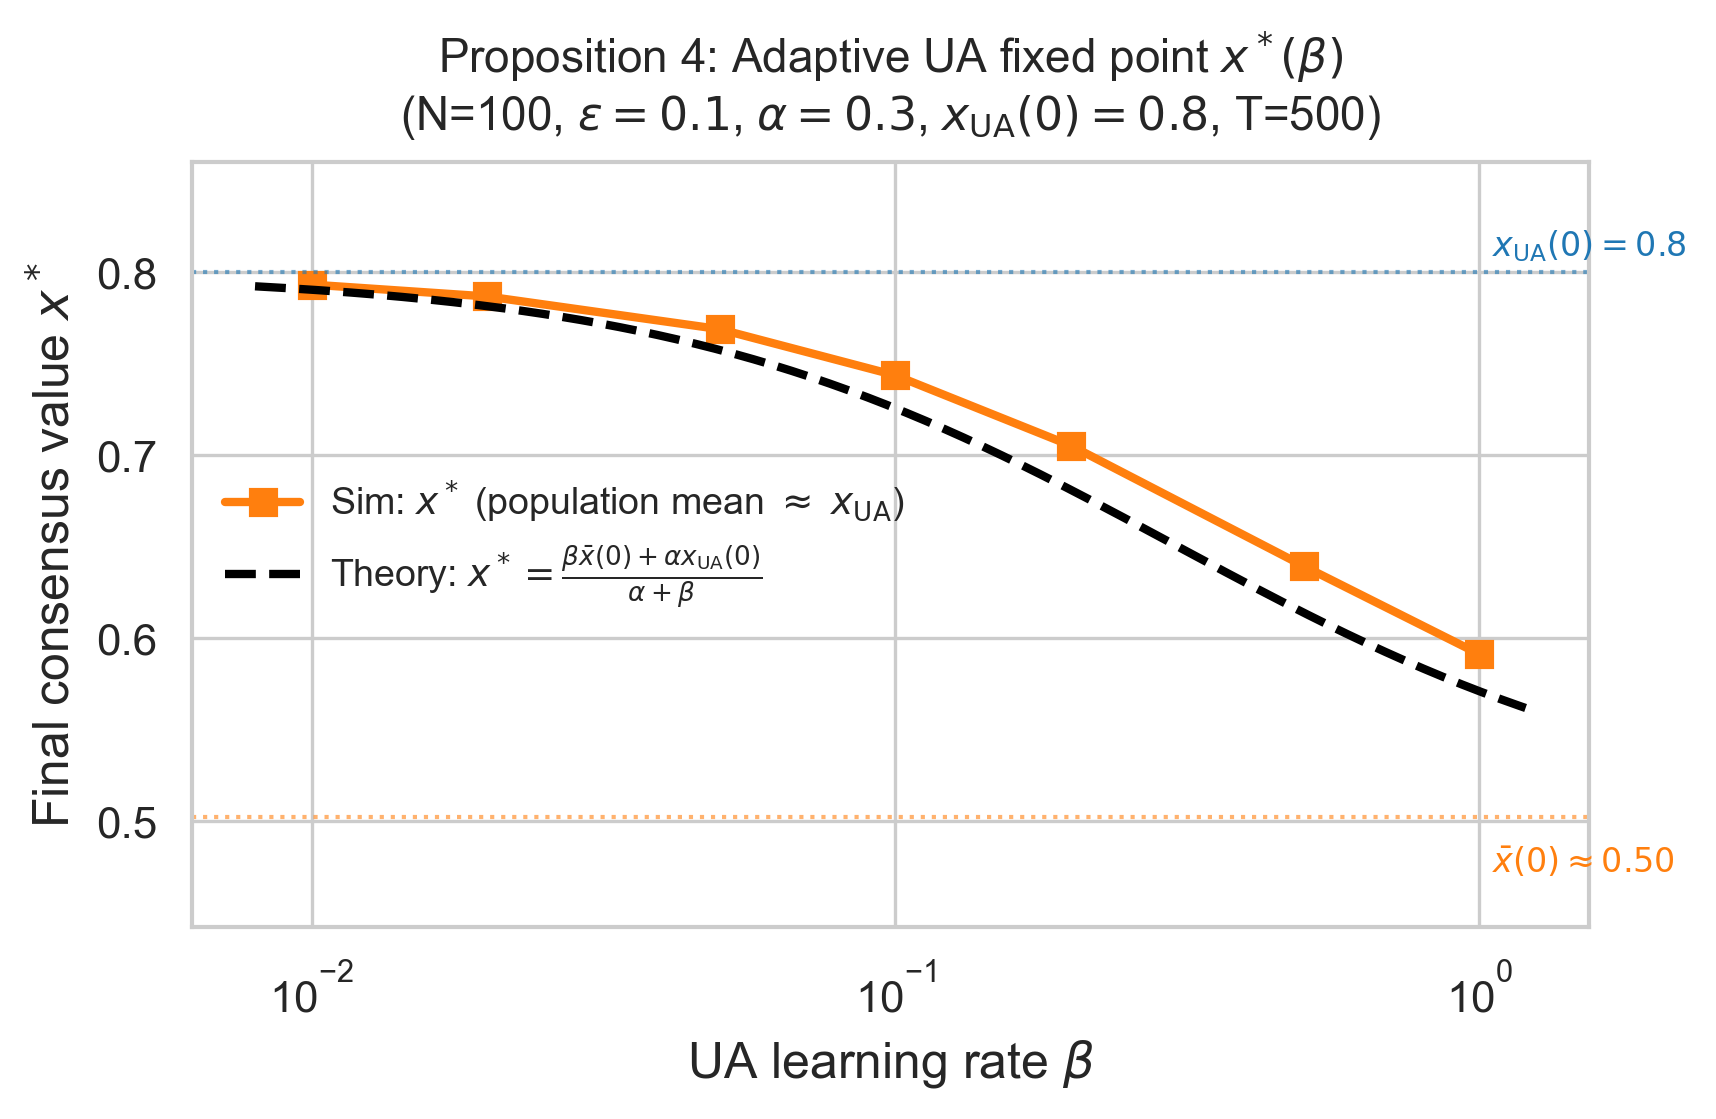
\includegraphics[width=\columnwidth]{../simulation/figures/exp4_adaptive_ua.png}}
\caption{\textbf{Setup.}  Final consensus value $x^*$ as a function of
the UA learning rate $\beta$ (log scale) at fixed $\alpha=0.3$,
$\varepsilon=0.1$, $\xUA(0)=0.8$.  Orange squares: simulation.
Dashed black: closed-form~\eqref{eq:xstar}.  Horizontal dotted
lines: limiting values $\xUA(0)$ ($\beta\to 0$) and $\xbar(0)$
($\beta\to 1$).}
\label{fig:setup}
\end{center}
\vskip -0.2in
\end{figure}

\subsection{R1 Validation: HK Cluster Breaking}

We sweep $\alpha$ on a log grid from $10^{-3}$ to~$1$ at
$\varepsilon\in\{0.1,0.15,0.2\}$ with $\beta=0$ (the worst case for
cluster preservation, where the UA is purely fixed).
Figure~\ref{fig:R2_variance} reports the normalized asymptotic
variance $\Var(\infty)/\Var_0$.  Each curve drops sharply at the
empirical critical coupling $\hat\alpha^*\approx 0.001$--$0.003$,
far below the conservative upper bound
\eqref{eq:alphastar}---empirical evidence for the cascade mechanism
discussed in Remark~\ref{rem:R2_ratio}.  Figure~\ref{fig:R2_heatmap}
shows the same transition as a $(\alpha,\varepsilon)$ heat map.

\begin{figure}[ht]
\vskip 0.15in
\begin{center}
\centerline{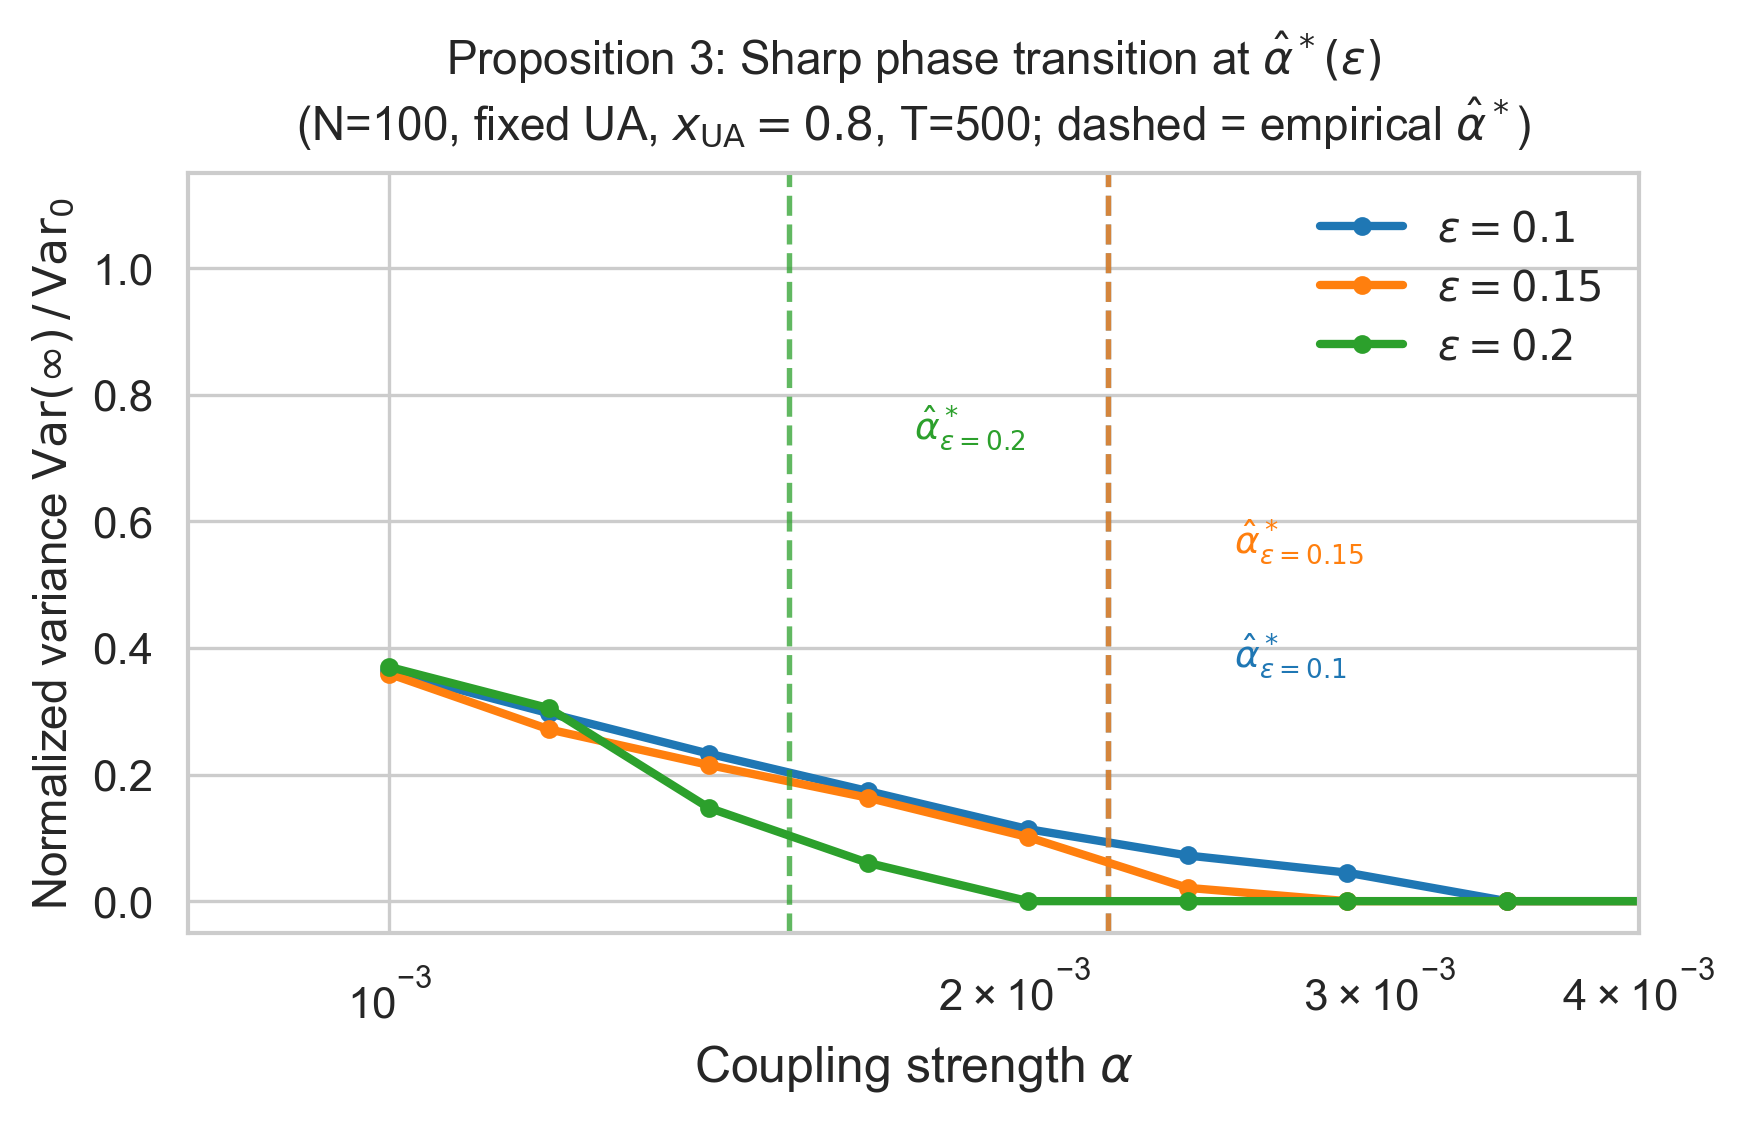
\includegraphics[width=\columnwidth]{../simulation/figures/exp2_variance_vs_alpha.png}}
\caption{\textbf{R2.}  Normalized asymptotic variance vs.\ coupling
$\alpha$ for HK with a fixed UA ($\beta=0$), $\xUA=0.8$, $N=100$.
A sharp drop occurs at $\hat\alpha^*\approx 0.001$--$0.003$ for
$\varepsilon\in\{0.1,0.15,0.2\}$; dashed lines mark the empirical
$\hat\alpha^*$ per curve.}
\label{fig:R2_variance}
\end{center}
\vskip -0.2in
\end{figure}

\begin{figure}[ht]
\vskip 0.15in
\begin{center}
\centerline{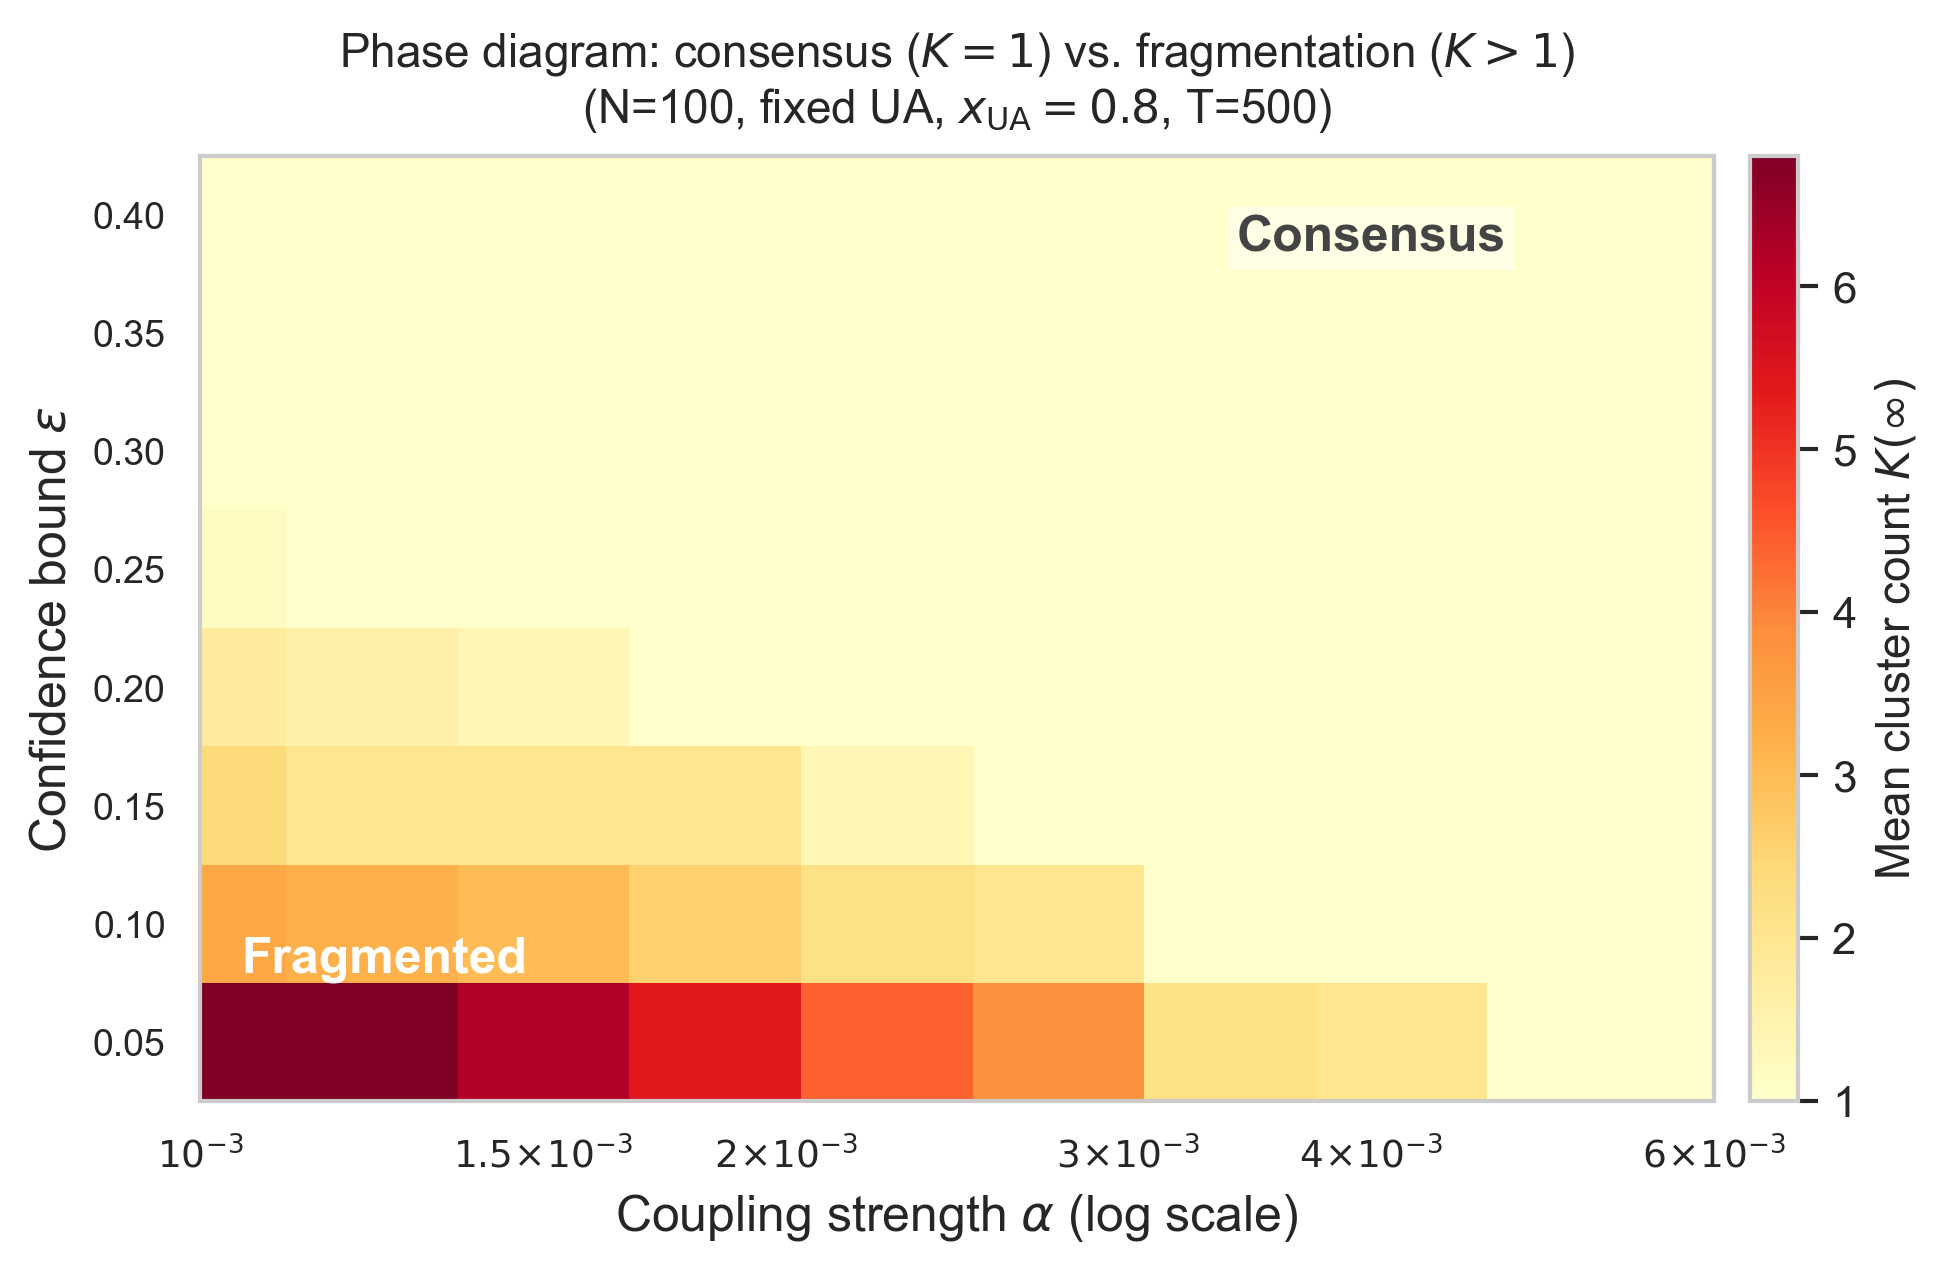
\includegraphics[width=\columnwidth]{../simulation/figures/exp3_phase_transition_heatmap.png}}
\caption{\textbf{R2.}  Heat map of the asymptotic cluster count
$K(\infty)$ in the $(\alpha,\varepsilon)$ plane (log~$\alpha$).
Dark = consensus; bright = fragmented.  The boundary traces the
empirical critical coupling $\hat\alpha^*(\varepsilon)$.}
\label{fig:R2_heatmap}
\end{center}
\vskip -0.2in
\end{figure}

The role of $\beta$ in HK can be read indirectly from
Figure~\ref{fig:R1}: as $\beta$ grows at fixed $\alpha=0.3$, the
final consensus moves away from $\xUA(0)$ and toward $\xbar(0)$.
A symmetric statement holds at smaller $\alpha$ near $\alpha^*$:
increasing $\beta$ erodes the UA's anchoring power and pushes the
threshold for cluster breaking outward.

\subsection{R2 Validation: Multiple UAs, Global vs.\ Local Adaptation}

We instantiate $k=4$ UAs, evenly spaced at
$u_j(0)\in\{0.1,0.35,0.65,0.9\}$, each interacting with $N/k=25$
agents under HK ($\varepsilon=0.1$, $\alpha=0.3$, $N=100$).
Figure~\ref{fig:R3_fixed} (Panel~A) confirms that fixed UAs
($\beta=0$) produce a permanent $K=4$ cluster configuration centred
on the UA positions.  Figure~\ref{fig:R3_adapt} (Panel~B) is the
central R3 plot: at $\beta=0.01$ for all four UAs, \emph{global}
adaptation collapses the four clusters to a single consensus by
$t\approx 160$, while \emph{local} adaptation preserves four
clusters indefinitely, matching the partition-specific equilibria
\eqref{eq:R3_local}.  The contrast is striking: at the same
$\alpha,\beta$, simply changing the target of UA adaptation
determines whether AI ecosystem diversity collapses or persists.

\begin{figure}[ht]
\vskip 0.15in
\begin{center}
\centerline{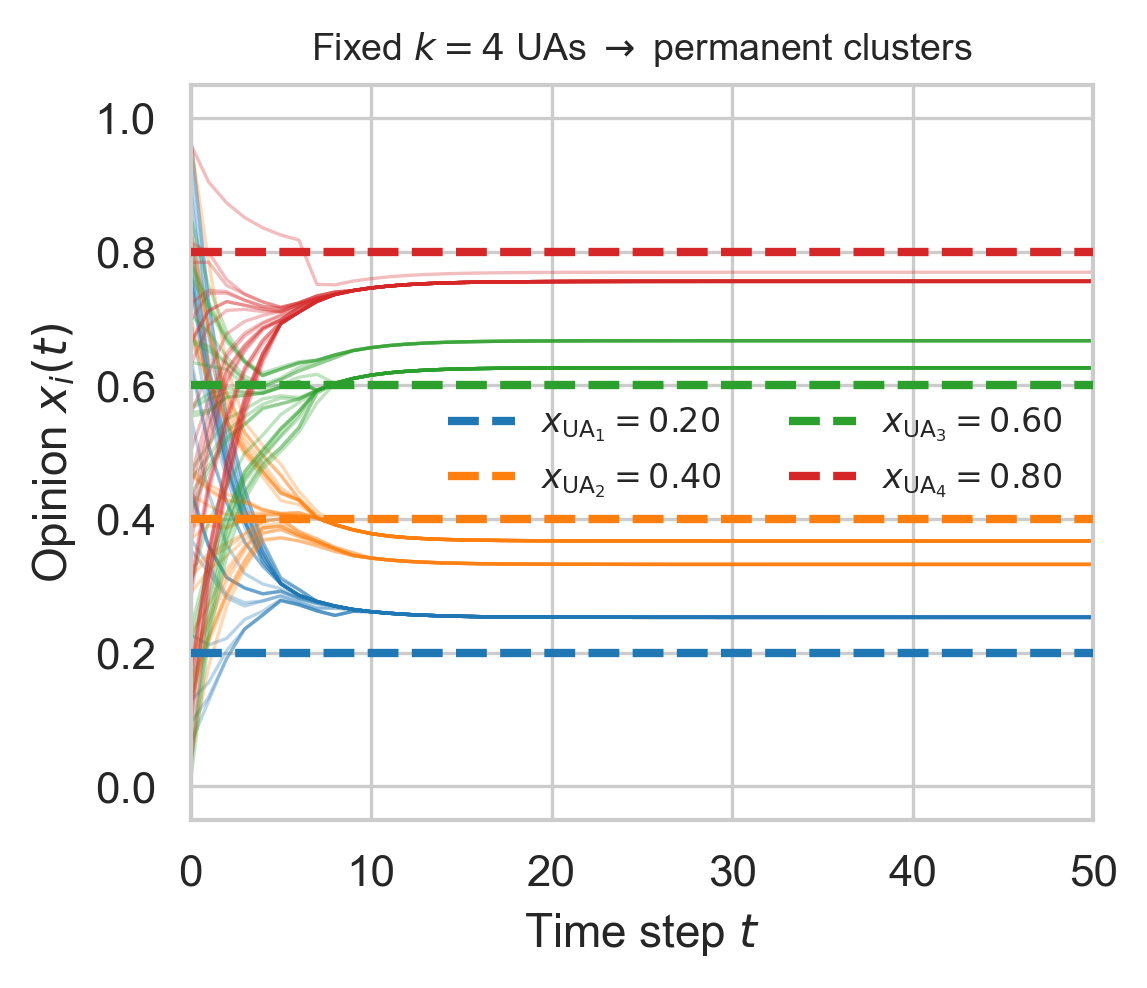
\includegraphics[width=\columnwidth]{../simulation/figures/exp6_multiple_ua_A.png}}
\caption{\textbf{R3 (A).}  Four fixed UAs at $u_j\in\{0.20,0.40,0.60,0.80\}$
produce permanent $K=4$ clusters anchored at the UA positions
($N=100$, $\varepsilon=0.1$, $\alpha=0.3$).}
\label{fig:R3_fixed}
\end{center}
\vskip -0.2in
\end{figure}

\begin{figure}[ht]
\vskip 0.15in
\begin{center}
\centerline{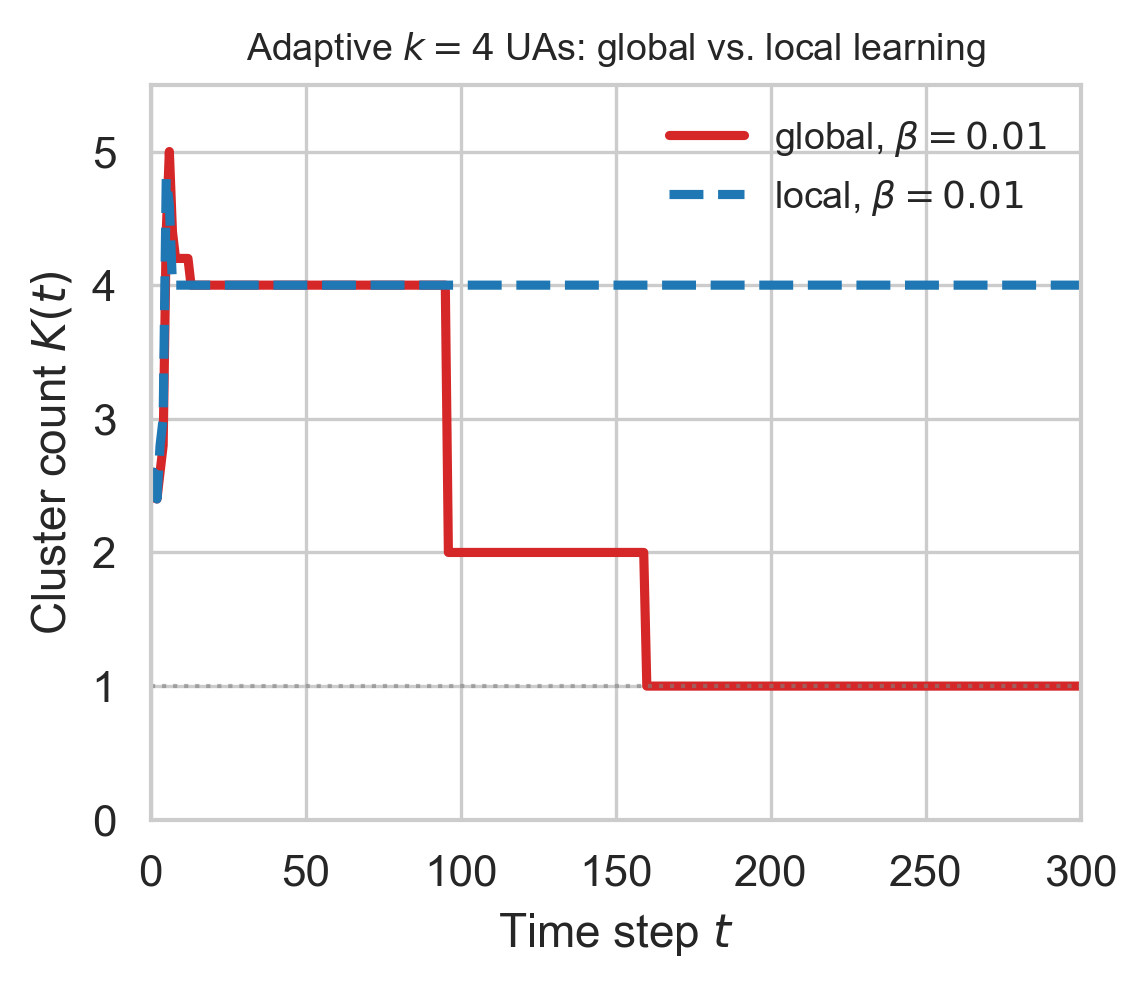
\includegraphics[width=\columnwidth]{../simulation/figures/exp6_multiple_ua_B.png}}
\caption{\textbf{R3 (B).}  Cluster count $K(t)$ for $k=4$ adaptive
UAs at $\beta=0.01$.  Global adaptation (solid red) collapses
$K\colon 4\to 1$ by $t\approx 160$; local adaptation
(dashed blue) preserves $K=4$ indefinitely, in agreement with
Theorem~\ref{thm:R3}(b).}
\label{fig:R3_adapt}
\end{center}
\vskip -0.2in
\end{figure}

\subsection{R3 Validation: Heterogeneous Reliance}

Finally we verify Proposition~\ref{prop:R4} under HK with $N=100$,
$\varepsilon=0.1$, $\xUA=0.8$.  Panel~A of Figure~\ref{fig:R4} shows
a representative trajectory for a bimodal $P(\alpha)$ with $50\%$
of agents at $\alpha_i=0.60$ and $50\%$ at $\alpha_i=0$: high-$\alpha$
agents (red) snap to $\xUA$ within $t\approx 3$ steps, whereas
low-$\alpha$ agents (blue) remain in peer clusters.  Panel~B
compares four reliance distributions: the no-UA baseline and both
bimodal distributions sustain $K\approx 3.4$--$3.8$ clusters, while
a heavy-tail distribution $\mathrm{Beta}(0.5,2)$ collapses to
$K=1$.  A skewed reliance pattern---even one whose mean coupling is
\emph{lower} than the bimodal cases---can therefore be \emph{more}
homogenizing than higher-mean alternatives, because its tail of
heavy users seeds a cascade.

\begin{figure}[ht]
\vskip 0.15in
\begin{center}
\centerline{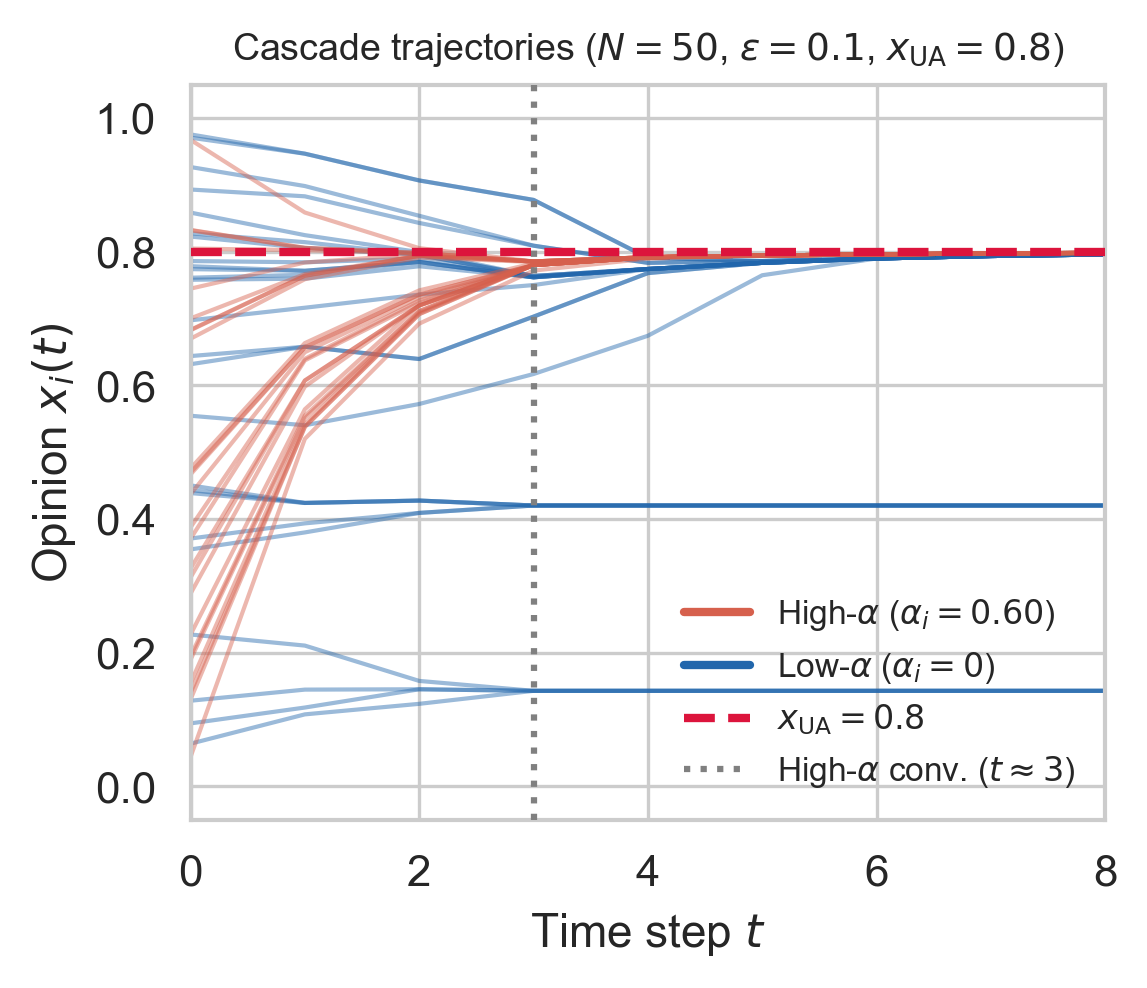
\includegraphics[width=\columnwidth]{../simulation/figures/exp5_heterogeneous_A.png}}
\caption{\textbf{R4 (A).}  Cascade trajectories under bimodal
$P(\alpha)$ ($50\%$ at $\alpha_i=0.60$, $50\%$ at $\alpha_i=0$;
$N=50$, $\varepsilon=0.1$, $\xUA=0.8$). High-$\alpha$ agents converge
within $t\approx 3$; low-$\alpha$ agents persist in peer clusters.}
\label{fig:R4}
\end{center}
\vskip -0.2in
\end{figure}

\begin{figure}[ht]
\vskip 0.15in
\begin{center}
\centerline{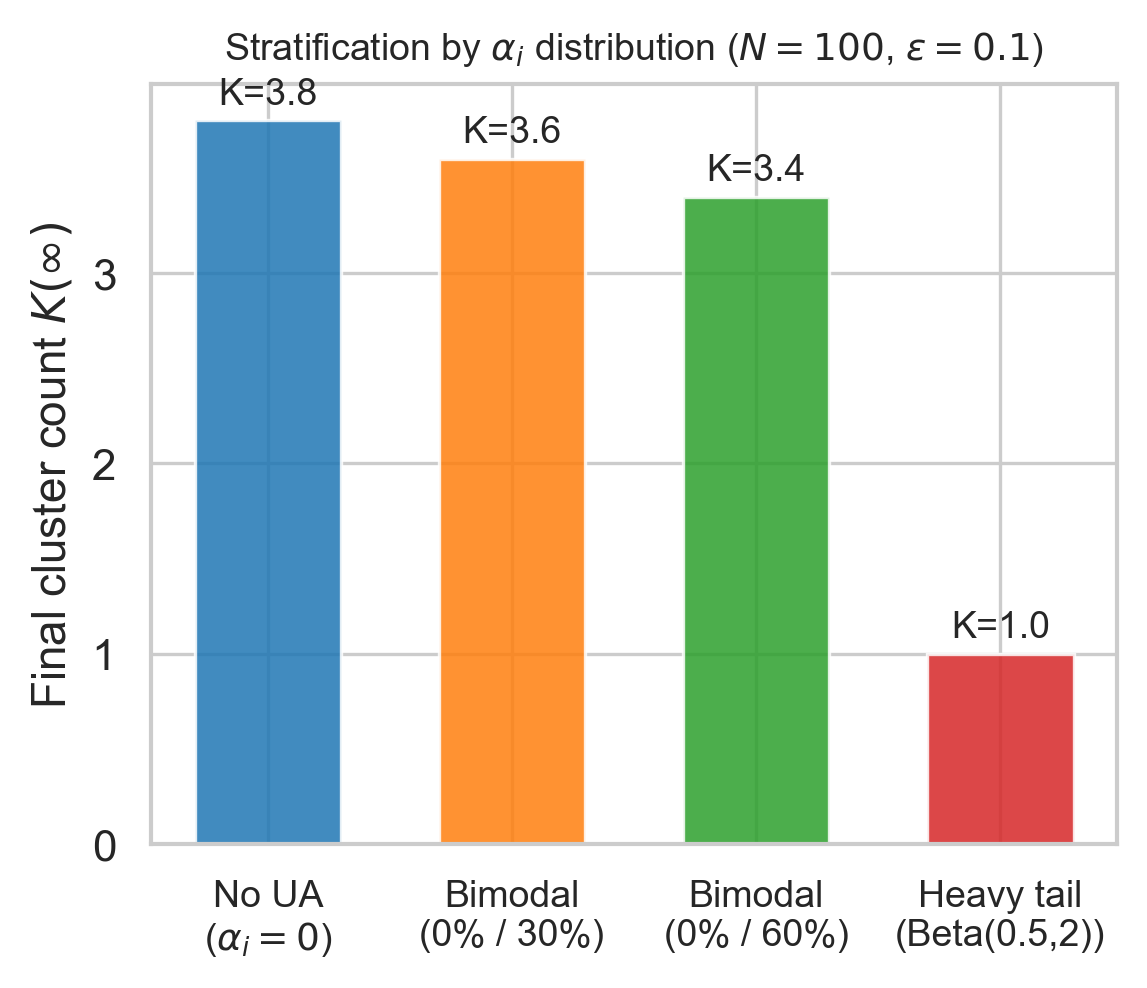
\includegraphics[width=\columnwidth]{../simulation/figures/exp5_heterogeneous_B.png}}
\caption{\textbf{R4 (B).}  Final cluster count $K(\infty)$ under
four reliance distributions ($N=100$, $\varepsilon=0.1$,
$\xUA=0.8$): no UA, bimodal $0\%/30\%$, bimodal $0\%/60\%$, and a
heavy-tail $\mathrm{Beta}(0.5,2)$.  The heavy tail collapses to
$K=1$ despite a lower mean $\bar\alpha$ than either bimodal case.}
\label{fig:R4_bar}
\end{center}
\vskip -0.2in
\end{figure}

%% ============================================================
\section{Discussion}
\label{sec:discussion}

\subsection{The $\alpha/\beta$ Ratio as a Design Lever}

Across all four results the ratio $\alpha/\beta$ controls
qualitative behaviour.  In DeGroot it determines the destination of
consensus (R1); in HK it determines whether the UA can break stable
clusters (R2); in the multi-UA setting under global adaptation it
controls the speed at which AI diversity collapses, and the
persistence weights $p_j/\beta_j$ determine which AI dominates the
final consensus (R3); under heterogeneous reliance it governs the
length of the cascade (R4).  Real LLMs sit firmly in the
$\alpha\gg\beta$ regime: a single retraining cycle costs months,
while inference-time influence is paid out across billions of
interactions per day.  In our framework this is exactly the
``slow-AI, anchoring'' regime, and the homogenization implications
follow directly.

\subsection{Governance Implications}

Two governance levers fall out of the analysis.  First, the
empirical $\alpha^*$ is small ($10^{-3}$ in our parameter regime),
which means any policy that aims to ``cap AI influence'' must do so
quantitatively---the relevant quantity is the joint distribution of
$\alpha_i$ across the user population, not the existence or absence
of an AI ``cap.''  Second, R3 suggests that even a market of many
nominally distinct LLMs can homogenize if their adaptation targets
are effectively shared (e.g.\ all retrained on overlapping web-scale
corpora): global adaptation collapses pluralism regardless of how
many AIs are nominally in the ecosystem.  Local
adaptation---per-region, per-community fine-tuning whose targets do
\emph{not} pool across all users---preserves multi-cluster equilibria
analytically.  A robust diversity policy should therefore favour
ecosystem designs in which AIs adapt to disjoint subpopulations, not
merely brand-distinct AIs trained on the same data.

\subsection{Stratification by Reliance}

R4 identifies an additional axis: AI-induced cultural stratification
by usage intensity.  The transient ``AI-aligned vanguard'' of heavy
users is observable in our simulations within a few time steps, and
the same mechanism explains why the empirical $\alpha^*$ is orders of
magnitude smaller than the two-cluster bridging bound: once a small
group is recruited, it acts as a peer-side bridge for the rest of the
population, lowering the effective coupling needed to break clusters.

\subsection{Limitations}

We work in one opinion dimension; multi-dimensional opinion space may
exhibit qualitatively different alignment phenomena (e.g.\ the UA
could induce consensus along some axes while preserving variation
along others).  Our peer dynamics are fully rational; bounded
rationality, motivated reasoning, and network-mediated trust are
absent.  Empirical calibration of $\alpha$ and $\beta$ from
real-world LLM interaction data is a major open problem and would
allow our thresholds to be compared against observed regimes.
Finally, R3(a) is proved in the partition-local reduction, which is
exact for block-structured peer networks and asymptotically correct
in HK once partitions separate; the joint dynamics with
not-yet-separated partitions in HK are studied only numerically.

%% ============================================================
\section{Conclusion}
\label{sec:conclusion}

We introduced an adaptive Universal Agent model of opinion dynamics
motivated by the deployment of LLMs as universal interlocutors, and
analysed it through four results.  In linear DeGroot dynamics a
single adaptive UA produces an exact closed-form consensus whose
location is governed by the ratio $\alpha/\beta$; in HK the same UA
breaks otherwise stable clusters once $\alpha/\beta$ is large enough
to make the UA effectively fixed; with multiple UAs, global
adaptation collapses pluralism to a weighted single consensus while
local adaptation preserves $k$ partition-specific equilibria; and
heterogeneous reliance produces a stratification cascade in which
heavy users homogenize first and seed the collapse of the rest.

Throughout, $\alpha/\beta$ and the locality of AI adaptation are the
twin design levers that determine whether deployed AI systems anchor
opinion, reflect it, or preserve a diverse equilibrium.  Promising
directions for future work include multi-dimensional opinion
geometry, empirical estimation of $\alpha$ and $\beta$ from
interaction logs, and network effects on the joint distribution of
$\alpha_i$ across populations.

\section*{Impact Statement}

This paper analyses cultural homogenization induced by universally
deployed AI systems.  The findings have direct societal implications:
the closed-form consensus formula identifies the AI adaptation rate
$\beta$ as a first-class governance variable alongside the coupling
$\alpha$, and the multi-UA result shows that nominal model diversity
does not preserve population-level pluralism unless adaptation
targets are also disjoint.  We advocate for regulatory mechanisms
that measure the joint $(\alpha,\beta)$ distribution and that
preferentially encourage locally-adapted AI ecosystems.

%% ============================================================
\begin{thebibliography}{99}

\bibitem[Acemoglu and Ozdaglar(2011)]{acemoglu2011}
Acemoglu, D., \& Ozdaglar, A. (2011).
Opinion dynamics and learning in social networks.
\textit{Dynamic Games and Applications}, 1(1), 3--49.

\bibitem[Acemoglu et al.(2013a)]{acemoglu2013degroot}
Acemoglu, D., Como, G., Fagnani, F., \& Ozdaglar, A. (2013).
Opinion fluctuations and disagreement in social networks.
\textit{Mathematics of Operations Research}, 38(1), 1--27.

\bibitem[Acemoglu et al.(2013b)]{acemoglu2013binary}
Acemoglu, D., Ozdaglar, A., Yildiz, E., Saberi, A., \& Scaglione, A. (2013).
Binary opinion dynamics with stubborn agents.
\textit{ACM Transactions on Economics and Computation}, 1(4), 19.

\bibitem[Barber\'{a}(2019)]{barbera2019}
Barber\'{a}, P. (2019).
Social media, echo chambers, and political polarization.
In N.~Persily \& J.~Tucker (Eds.),
\textit{Social Media and Democracy}.
Cambridge University Press.

\bibitem[Bernardo et al.(2024)]{bernardo2024}
Bernardo, C., et al. (2024).
Bounded confidence opinion dynamics: A survey.
\textit{Automatica}, 159, 111302.

\bibitem[Castellano et al.(2009)]{castellano2009}
Castellano, C., Fortunato, S., \& Loreto, V. (2009).
Statistical physics of social dynamics.
\textit{Reviews of Modern Physics}, 81(2), 591--646.

\bibitem[Centola et al.(2018)]{centola2018}
Centola, D., Becker, J., Brackbill, D., \& Baronchelli, A. (2018).
Experimental evidence for tipping points in social convention.
\textit{Science}, 360(6393), 1116--1119.

\bibitem[Chica et al.(2023)]{chica2023}
Chica, M., et al. (2023).
Modelling opinion dynamics under the impact of influencer and media strategies.
\textit{Scientific Reports}, 13, 19198.

\bibitem[Crokidakis and de Oliveira(2014)]{crokidakis2014}
Crokidakis, N., \& de Oliveira, P.~M.~C. (2014).
Evolution of public opinions in closed societies influenced by broadcast media.
\textit{Physica~A}.

\bibitem[Daryani et al.(2026)]{daryani2026}
Daryani, Y., Sourati, Z., \& Dehghani, M. (2026).
The homogenizing engine: AI's role in standardizing culture and the path to policy.
\textit{Social Media + Society}.

\bibitem[DeGroot(1974)]{degroot1974}
DeGroot, M.~H. (1974).
Reaching a consensus.
\textit{Journal of the American Statistical Association}, 69(345), 118--121.

\bibitem[Deffuant et al.(2000)]{deffuant2000}
Deffuant, G., Neau, D., Amblard, F., \& Weisbuch, G. (2000).
Mixing beliefs among interacting agents.
\textit{Advances in Complex Systems}, 3(1--4), 87--98.

\bibitem[Friedkin and Johnsen(1990)]{friedkin1990}
Friedkin, N.~E., \& Johnsen, E.~C. (1990).
Social influence and opinions.
\textit{Journal of Mathematical Sociology}, 15(3--4), 193--206.

\bibitem[Galam(2002)]{galam2002}
Galam, S. (2002).
Minority opinion spreading in random geometry.
\textit{European Physical Journal B}, 25(4), 403--406.

\bibitem[Hegselmann and Krause(2002)]{hegselmann2002}
Hegselmann, R., \& Krause, U. (2002).
Opinion dynamics and bounded confidence: Models, analysis, and simulation.
\textit{Journal of Artificial Societies and Social Simulation}, 5(3), 2.

\bibitem[Lorenz(2007)]{lorenz2007}
Lorenz, J. (2007).
Continuous opinion dynamics under bounded confidence: A survey.
\textit{International Journal of Modern Physics C}, 18(12), 1819--1838.

\bibitem[Markl et al.(2025)]{markl2025}
Markl, A., et al. (2025).
AI suggestions homogenize writing toward Western styles and diminish cultural nuances.
\textit{Proceedings of CHI 2025}.

\bibitem[Mobilia(2003)]{mobilia2003}
Mobilia, M. (2003).
Does a single zealot affect an infinite group of voters?
\textit{Physical Review Letters}, 91(2), 028701.

\bibitem[Mobilia et al.(2007)]{mobilia2007}
Mobilia, M., Petersen, A., \& Redner, S. (2007).
On the role of zealotry in the voter model.
\textit{Journal of Statistical Mechanics}, P08029.

\bibitem[Pariser(2011)]{pariser2011}
Pariser, E. (2011).
\textit{The Filter Bubble: What the Internet Is Hiding from You}.
Penguin Press.

\bibitem[Pineda et al.(2022)]{pineda2022}
Pineda, M., Toral, R., \& Hern\'{a}ndez-Garc\'{i}a, E. (2022).
Noisy bounded confidence models for opinion dynamics.
\textit{IMA Journal of Applied Mathematics}, 87(1), 80--110.

\bibitem[Sharma et al.(2024)]{sharma2024}
Sharma, A., et al. (2024).
Generative echo chamber? Effects of LLM-powered search systems on diverse information seeking.
\textit{Proceedings of CHI 2024}.

\bibitem[Zhang et al.(2025)]{zhang2025}
Zhang, S., Xu, J., \& Alvero, A.~J. (2025).
Generative AI meets open-ended survey responses: Research participant use of AI and homogenization.
\textit{Sociological Methods \& Research}.

\end{thebibliography}

%% ============================================================
\clearpage
\appendix
\section{Proofs}
\label{app:proofs}

\subsection{Convergence rate for individual disagreement modes
(Theorem~\ref{thm:R1}, second statement)}

Write the single-UA DeGroot update in matrix form as
$\bx(t+1)=(1-\alpha)W\bx(t)+\alpha\,\xUA(t)\bone$.  For \emph{fixed}
$\xUA$ this is an affine map with linear part $M=(1-\alpha)W$.
Define the error $\mathbf{e}(t)=\bx(t)-\xUA\bone$ (or, for adaptive
$\xUA$, $\mathbf{e}(t)=\bx(t)-\xbar(t)\bone$ once aggregate
convergence is reached).  Subtracting the fixed-point equation from
the update gives $\mathbf{e}(t+1)=M\mathbf{e}(t)$, so
$\mathbf{e}(t)=M^t\mathbf{e}(0)=(1-\alpha)^t W^t \mathbf{e}(0)$.
Because $W$ is strongly connected and aperiodic,
$\|W^t\mathbf{e}(0)\|_\infty\le C\lambda_2(W)^t\|\mathbf{e}(0)\|_\infty$
for a constant $C$, hence
$\|\mathbf{e}(t)\|_\infty\le C[(1-\alpha)\lambda_2(W)]^t\|\mathbf{e}(0)\|_\infty$.

\subsection{Proof of Proposition~\ref{prop:R2} (HK critical coupling)}

Baseline HK at $\alpha=0$ on $\mathcal{U}[0,1]$ produces
$K\approx\lfloor 1/(2\varepsilon)\rfloor$ clusters.  Consider the
stylized two-cluster case with centroids $\mu_L\approx\varepsilon$
and $\mu_R\approx 1-\varepsilon$, separated by
$\Delta=\mu_R-\mu_L\approx 1-2\varepsilon$.  Under one HK+UA step
with $\xUA$ at the centre, each centroid moves to
$(1-\alpha)\mu_{L,R}+\alpha\xUA$, so the inter-centroid gap shrinks
to $(1-\alpha)\Delta$.  The clusters enter each other's confidence
window once $(1-\alpha)\Delta<\varepsilon$, giving the conservative
threshold
\[
    \alpha^*
    \;\le\; 1 - \frac{\varepsilon}{\Delta}
    \;=\; \frac{1-3\varepsilon}{1-2\varepsilon}.
\]
This is a one-step sufficient condition.  It ignores sequential
recruitment (Proposition~\ref{prop:R4}); once a small bridge of
agents reaches the UA, those agents act as peer-side anchors that
further reduce the effective $\Delta$, so the finite-population
transition is far below the bound.

\subsection{Proof of Theorem~\ref{thm:R3}(a) (Global adaptation)}

We verify that
\[
    Q(t) \;=\; \frac{1}{\alpha}\,\mbar(t)
        + \sum_{j=1}^{k} \frac{p_j}{\beta_j}\,u_j(t)
\]
is invariant.  Compute:
\begin{align*}
    \mbar(t+1)
    &= \sum_j p_j m_j(t+1)\\
    &= \sum_j p_j\big[(1-\alpha)m_j(t) + \alpha u_j(t)\big]\\
    &= (1-\alpha)\mbar(t) + \alpha\sum_j p_j u_j(t),
\end{align*}
so
$\frac{1}{\alpha}\mbar(t+1)
   = \frac{1}{\alpha}\mbar(t) - \mbar(t) + \sum_j p_j u_j(t)$.
For the UA term, since $\tau_j=\mbar(t)$,
\begin{align*}
    \sum_j \frac{p_j}{\beta_j} u_j(t+1)
    &= \sum_j \frac{p_j}{\beta_j}\Big[(1-\beta_j)u_j(t)+\beta_j\mbar(t)\Big]\\
    &= \sum_j \frac{p_j}{\beta_j}u_j(t) - \sum_j p_j u_j(t)
       + \mbar(t).
\end{align*}
Adding the two pieces, the $\sum_j p_j u_j(t)$ and $\mbar(t)$ terms
cancel and $Q(t+1)=Q(t)$.

The matrix governing $(m_1,\ldots,m_k,u_1,\ldots,u_k)$ is row-stochastic
on its $2k$ coordinates restricted to the conserved hyperplane, with
unit spectral radius once and contracting elsewhere (the analogue of
the $2\times 2$ argument used in Theorem~\ref{thm:R1}, repeated
$k$~times with coupling through $\mbar$).  Therefore all $m_j(t)$
and $u_j(t)$ converge to a common limit $x^*$, and equating $Q$ with
$x^*\,(\frac{1}{\alpha}+\sum_j p_j/\beta_j)$ yields
\eqref{eq:R3_global}.

Part (b) follows by applying Theorem~\ref{thm:R1} to each partition
independently, since under local adaptation $\tau_j=m_j$ the system
decouples across~$j$.

\subsection{Proof of Proposition~\ref{prop:R4} (Stratification cascade)}

For fixed $\xUA$, the system
$x_i(t+1) = (1-\alpha_i)\sum_j w_{ij}x_j(t)+\alpha_i\xUA$
has a unique fixed point $x_i^*=\xUA$ because the effective peer
operator $[(1-\alpha_i)w_{ij}]$ has row sums $1-\alpha_i<1$ for every
$i$, so the affine map is a contraction.  For the individual
convergence rate, once peers are close to their limit the dominant
relaxation is
$|e_i(t+1)|\le (1-\alpha_i)|e_i(t)|$,
giving $|e_i(t)|\le (1-\alpha_i)^t|e_i(0)|$.  Setting this to a
tolerance $\delta$ and using $\log(1-\alpha_i)\approx -\alpha_i$ for
small $\alpha_i$ yields
$T_i^*(\alpha_i)\approx\log(|e_i(0)|/\delta)/\alpha_i$,
which is \eqref{eq:Ti}.  The cascade statement is qualitative: as
high-$\alpha_i$ agents converge to $\xUA$, they enter the peer terms
of low-$\alpha_i$ agents, effectively raising the attraction toward
$\xUA$ for the remainder of the population.

\end{document}
